\section{Theory}

\begin{frame}{Motivations}
  \begin{block}{Algorithmic problems}
    \begin{itemize}
      \item Stochastic
      \item Convergence
    \end{itemize}
  \end{block}

  \begin{block}{Modelisation problems}
    \begin{itemize}
      \item How to encode a problem?
      \item Size of the initial population?
      \item Mutation operator?
      \item Recombination operator?
      \item Individual selection?
    \end{itemize}
  \end{block}
\end{frame}

\subsection{Schemata Theorem}
\begin{frame}{Presentation}
  \begin{block}{Goal}
    \begin{itemize}
    \item Defined by J.Holland in 1975\cite{holland1992}.
    \item Represent a group of indidual who all share some caracteristics.
    \item One schema, two schemata ;)
    \end{itemize}
  \end{block}    

  \begin{block}{Definition}
    \begin{itemize}
    \item Defined on the alphabet: $\{0;1;\#\}$
    \item $\#$ is "Don't care": it can be 0 or 1
    \end{itemize}
  \end{block}
\end{frame}

\begin{frame}{Example and mesures}
  \begin{block}{Example}
    \begin{itemize}
    \item The schema: $H = 1\textcolor{red}{\#}10\textcolor{red}{\#}1\textcolor{red}{\#}$
    \item Represents the following individuals:
      \begin{center}
        $1\textcolor{red}{0}10\textcolor{red}{0}1\textcolor{red}{0}$,
        $1\textcolor{red}{0}10\textcolor{red}{0}1\textcolor{red}{1}$,
        $1\textcolor{red}{0}10\textcolor{red}{1}1\textcolor{red}{0}$,
        $1\textcolor{red}{0}10\textcolor{red}{1}1\textcolor{red}{1}$,
        $1\textcolor{red}{1}10\textcolor{red}{0}1\textcolor{red}{0}$,
        $\ldots$
      \end{center}
    \end{itemize}
  \end{block}

  \begin{block}{Measures}
    \begin{itemize}
      \item Order(o): number of fixed positions
      \item Defining length($\delta$): distance between the first and last defined positions.
      \item Here: $o(H) = 4$ and $\delta(H) = 5$
      \item Intuitively: schemata with low o and short $\delta$ have an higher probability of surviving from a generation to the next.
    \end{itemize}
  \end{block}
\end{frame}

\begin{frame}{Graphical representation}
  \begin{center}
    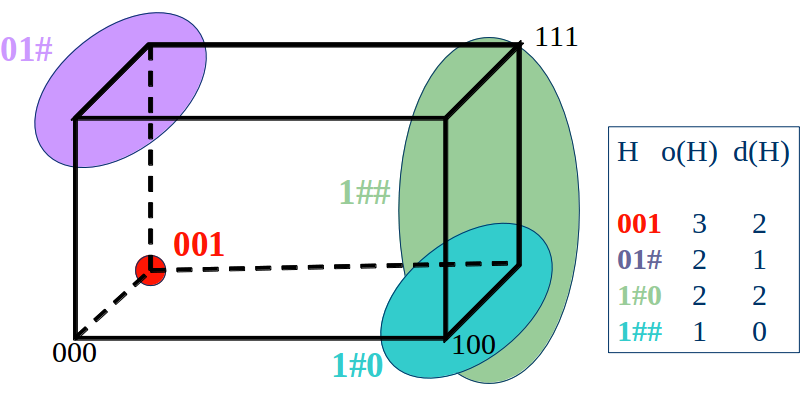
\includegraphics[scale=.4]{img/schema}
  \end{center}
\end{frame}

\begin{frame}{Possible evolutions : selection}
  \begin{block}{Hypothesis}
    \begin{itemize}
    \item Assume a fitness proportional reproduction
    \item $$\mathds{P}(x,t+1) = \frac{f(x)}{\bar{f(t)}}$$
    \end{itemize}
  \end{block}

  \begin{block}{Transmission of a schema}
    $$\begin{array}{lll}
      \mathds{P}(H,t+1) & = & \sum\limits_{x \in H} \frac{f(x)}{\bar{f(t)}}\\
      & = & m(H,t) \times \frac{f(H,t)}{\bar{f(t)}}\\
    \end{array}$$
  \end{block}
\end{frame}

\begin{frame}{Disruptions}
  \begin{block}{Mutation}
    \begin{itemize}
    \item bit-wise mutations with probability $p_m$
    \item Mutation events are independant
    \item $\mathds{P}_{Smuta}(H) \geq (1 - p_m)^{o(H)}$
    \end{itemize}
  \end{block}

  \begin{block}{Crossover}
    \begin{itemize}
      \item One point crossover with probability $p_c$
      \item l - 1 possible crossover points
      \item $\mathds{P}_{Scross}(H) \geq (1 - p_c \times \frac{\delta(H)}{l - 1})$
    \end{itemize}
  \end{block}
\end{frame}

\begin{frame}{Schema theorem}
  \begin{block}{Theorem}
    $$E(m(H,t+1)) \geq \underbrace{m(H,t) \times \frac{f(H,t)}{\bar{f(t)}}}_{\mathds{P}(x,t+1)}
    \underbrace{\times (1 - p_c \times \frac{\delta(H)}{l-1})\vphantom{\frac{f(H,t)}{\bar{f(t)}}}}_{\mathds{P}_{Smuta}}
    \underbrace{\times (1 - p_m)^{o(H)}\vphantom{\frac{f(H,t)}{\bar{f(t)}}}}_{\mathds{P}_{Scross}}$$
  \end{block}
\end{frame}

\begin{frame}{Extension to GP}
\end{frame}

\begin{frame}{Building Block hypothesis}
\end{frame}

\begin{frame}{Price's theorem}
\end{frame}

\begin{frame}{Limitations}
\end{frame}

\begin{frame}{Conclusion}
\end{frame}
